% !TeX spellcheck = en_GB

\subsection{\acrfull{svm}}
\label{subsection:svm}

	Considering instances of data with their respective ground-truth labels, this classifier finds the frontier defined as a hyperplane that maximizes the distance between the two observations closest to each other that belong to different classes and are more likely to be misclassified. These two points are called support vectors \cite{Fu2011}. In order to find this hyperplane, the data is mapped into a higher dimensional space so it can be more separable. This is done by applying a kernel function that eases the process of finding a proper mapping function. Some of the most used ones are the polynomial, Gaussian, linear, sigmoid and \acrshort{rbf} \cite{Bhattacharyya2018}.
	
	This type of method is characterized for being a binary classifier. However, its implementation has been transported to multiclass problems by combining various \acrshort{svm}s in order to establish a decision criterion so the whole system can chose among $Q$ categories. This can be done by following either one-versus-all or one-versus-one approach. The former addresses the problem training $Q$ classifiers so as to differentiate between data from one class and data from the other $Q-1$ classes. The latter treats the problem by training $\frac{Q(Q-1)}{2}$ \acrshort{svm}s to distinguish among all possible combinations of categories. In any of the approaches, the classification of a certain observation is performed by computing the distance between the sample data and the hyperplane that defines the frontier \cite{Barchiesi2015}. 
	
	The one-versus-one is the one implemented by \acrfull{svc} from Scikit-learn library and is the one we will use in one of the experiments explained in section \ref{subsection:implementation-1}. In figure \ref{fig:mesh10} it is shown a representation of the decision boundaries that could be designed by other type of methods against the hyperplane a \acrshort{svm} classifier would draw.
	
	\begin{figure}[H]
		\centering
		\captionsetup{justification=centering}
		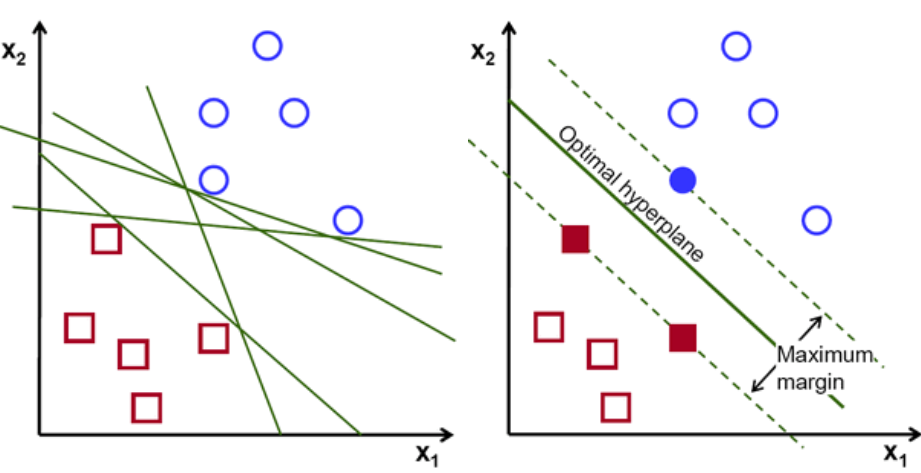
\includegraphics[scale=0.2]{svm}
		\caption{Visualization of a hyperplane set by \acrshort{svm} and other decision boundaries \cite{Drakos2018}}
		\label{fig:mesh10}
	\end{figure}
